\documentclass[UTF8,12pt]{article} % 12pt 为字号大小
\usepackage{amssymb,amsfonts,amsmath,amsthm}
\usepackage{times}
\usepackage{graphicx} % 插图
\usepackage{cite}
\usepackage{ctex}
\usepackage{color}
\usepackage{caption}
\usepackage{placeins} % 防止浮动
%----------
% 插入代码的格式定义
% 参考 https://www.latexstudio.net/archives/5900.html
%----------
\usepackage{listings}
\lstset{
 columns=fixed,       
 numbers=left,                                        % 在左侧显示行号
 numberstyle=\tiny\color{gray},                       % 设定行号格式
 frame=none,                                          % 不显示背景边框
 backgroundcolor=\color[RGB]{245,245,244},            % 设定背景颜色
 keywordstyle=\color[RGB]{40,40,255},                 % 设定关键字颜色
 numberstyle=\footnotesize\color{darkgray},           
 commentstyle=\it\color[RGB]{0,96,96},                % 设置代码注释的格式
 stringstyle=\rmfamily\slshape\color[RGB]{128,0,0},   % 设置字符串格式
 showstringspaces=false,                              % 不显示字符串中的空格
 language=c++,                                        % 设置语言
}
%----------
% 算法伪代码
% https://blog.csdn.net/lwb102063/article/details/53046265
%----------
\usepackage{algorithm}  
\usepackage{algpseudocode}  
\usepackage{amsmath}  
\renewcommand{\algorithmicrequire}{\textbf{Input:}}  % Use Input in the format of Algorithm  
\renewcommand{\algorithmicensure}{\textbf{Output:}} % Use Output in the format of Algorithm  

%----------
% 字体定义
%----------

\newcommand*{\kaiti}{\CJKfamily{zhkai}}  % 楷体
\newcommand*{\yuanti}{\CJKfamily{zhyou}} % 圆体

%----------
% 版面设置
%----------
%首段缩进
\usepackage{indentfirst}
\setlength{\parindent}{2em}
%行距
\renewcommand{\baselinestretch}{1.25} % 1.25倍行距
%页边距
\usepackage[a4paper]{geometry}
\geometry{verbose,
  tmargin=2cm,% 上边距
  bmargin=2cm,% 下边距
  lmargin=2cm,% 左边距
  rmargin=2cm % 右边距
}

% ----------
% 多级标题格式在此设置
% https://zhuanlan.zhihu.com/p/32712209
% \titleformat{command}[shape]%定义标题类型和标题样式,字体
% {format}%定义标题格式:字号(大小),加粗,斜体
% {label}%定义标题的标签,即标题的标号等
% {sep}%定义标题和标号之间的水平距离
% {before-code}%定义标题前的内容
% [after-code]%定义标题后的内容
% ----------
\usepackage{titlesec} %自定义多级标题格式的宏包
% 三级标题
% 4
\titleformat{\section}[block]{\large \bfseries}{\arabic{section}}{1em}{}[]
% 4.1
\titleformat{\subsection}[block]{\normalsize \bfseries}{\arabic{section}.\arabic{subsection}}{1em}{}[]
% 4.1.1
\titleformat{\subsubsection}[block]{\small \mdseries}{\arabic{section}.\arabic{subsection}.\arabic{subsubsection}}{1em}{}[]
\titleformat{\paragraph}[block]{\footnotesize \bfseries}{[\arabic{paragraph}]}{1em}{}[]


%----------
% 其他宏包
%----------
%图形相关
\usepackage[x11names]{xcolor} % must before tikz, x11names defines RoyalBlue3
\usepackage{graphicx}
\usepackage{pstricks,pst-plot,pst-eps}
\usepackage{subfig}
\def\pgfsysdriver{pgfsys-dvipdfmx.def} % put before tikz
\usepackage{tikz}

%原文照排
\usepackage{verbatim}

%链接的格式
\usepackage[colorlinks,linkcolor=red]{hyperref}
%表格
\usepackage{tabularx}

%==========
% 正文部分
%==========
\captionsetup[figure]{labelsep=period}
\captionsetup[table]{labelsep=period}

\begin{document}

\title{\bf{A Recurrent Network Model of Planning Explains Hippocampal Replay and Human Behavior}}
\author{Kristopher T. Jensen, Guillaume Hennequin, Marcelo G. Mattar}
\date{July 2024}
\begin{titlepage}
%本页为自定义的封面
	\newcommand{\ID}{{\Large 000000000}}
	\newcommand{\supervisor}{{\Large XXX}}
    
	\center
	\quad\\[1cm]
	
\includegraphics[width=12cm]{Content/logo.jpg}\\[1.5cm]
	\quad\\[1cm]
	\makeatletter
	{\linespread{4}\Huge\bfseries 计算机前沿技术}\\[1cm]
{\linespread{4}\Huge\bfseries 研究生创新示范课程研究报告}\\[2cm]
	\begin{table}[H]
		\centering
		  \begin{tabular}{rl}
			{\Large 姓名:}&{\Large 徐吕恒}\\[1cm]
			{\Large 学号:}&{\Large 2410105005}\\[1cm]
		  \end{tabular}\\
	\end{table}
	\makeatother
	\quad\\[1cm]
	{\Large 2024年12月5日}\\[2cm] % 日期
	\vfill 
\end{titlepage} 
\maketitle
\begin{abstract}
	% \kaiti 是楷体,参见上面的字体设置
	{\kaiti When faced with a novel situation, people often spend substantial periods of time contemplating possible futures. For such planning to be rational, the benefits to behavior must compensate for the time spent thinking. Here, we capture these features of behavior by developing a neural network model where planning itself is controlled by the prefrontal cortex. This model consists of a meta-reinforcement learning agent augmented with the ability to plan by sampling imagined action sequences from its own policy, which we call ‘rollouts’. In a spatial navigation task, the agent learns to plan when it is beneficial, which provides a normative explanation for empirical variability in human thinking times. Additionally, the patterns of policy rollouts used by the artificial agent closely resemble patterns of rodent hippocampal replays. Our work provides a theory of how the brain could implement planning through prefrontal–hippocampal interactions, where hippocampal replays are triggered by—and adaptively affect—prefrontal dynamics.}
 	\\\\
 	\textbf{Key Wrods:}planning, hippocampal replay, prefrontal cortex, decision-making
\end{abstract}

\section{引言}

在面对新情况时,人们往往会花费大量时间思考可能的未来。这种规划行为需要在行为上的收益与思考时间之间达到平衡。本文通过开发一个神经网络模型,探讨了前额叶皮层如何控制规划过程,以及海马体重放与人类行为之间的关系,为理解大脑如何实现规划提供了新的理论基础

\section{相关工作}
	此部分对课题内容相关的工作进行简要的分类概括与描述,二级标题中的内容为示意,可按照行文内容进行增删与更改,若二级标题无法对描述内容进行概括,可自行增加三级标题,后面内容同样如此,引文的bib文件统一粘贴到\textbf{refs.bib}中并采用如下引用方式~\cite{liu_2024_brep}。

	在认知控制和决策制定领域,已有研究从多个角度探讨了大脑活动与行为表现之间的关系。Fischer等人通过研究皮质β波功率,揭示了决策动态以及错误后适应的多个方面 \cite{Fischer_Nigbur_Klein_Danielmeier_Ullsperger_2018}。他们发现,皮质β波功率不仅反映了决策过程中的动态变化,还能 uncover 错误后适应的多个维度,为理解大脑如何在错误后调整认知控制提供了新的视角。

	Froemer等人则关注了奖励预期和效能感如何引导认知控制的分配\cite{Froemer_Lin_Dean_Wolf_Inzlicht_Shenhav_2021}。他们的研究表明,个体对奖励的预期以及对自己行动效能的感知,在认知控制资源的分配中起着关键作用。这一发现强调了在复杂决策情境中,个体的主观预期和自我效能感对行为调节的重要性。
	
	此外,Froemer等人进一步探讨了目标一致性与奖励价值在价值基础决策中的作用\cite{Froemer_Dean_Wolf_Shenhav_2019} 。研究指出,目标一致性在解释行为和神经相关性方面,比奖励价值具有更强的影响力。这表明,在决策过程中,个体不仅考虑行动的潜在奖励,还会评估行动与自身目标的契合度,从而做出更符合自身长期目标的选择。
	
	这些研究共同为我们理解大脑如何在动态环境中灵活调整认知控制和决策策略提供了重要的理论基础和实证支持。通过整合这些研究成果,我们可以更深入地探讨在不同情境下,个体如何权衡奖励、目标一致性和自我效能感等因素,以实现最优的行为表现。

\section{本文方法}


\subsection{本文方法概述}
这篇文章中使用到的元强化学习模型是一个循环神经网络(RNN)模型,该模型通过采样自身的策略来生成想象中的行动序列(称为“rollouts”)来进行规划。这个模型由前额叶皮层控制,能够学习在何时进行规划,以补偿思考时间的消耗。模型的目标是在空间导航任务中,当规划有益时学习进行规划,这为人类思考时间的实证变异性提供了一个规范性的解释。此外,人工代理使用的策略rollouts模式与啮齿动物海马回放的模式非常相似。这个模型提供了一个理论,即大脑如何通过前额叶-海马体的相互作用来实现规划,其中海马回放由前额叶动态触发,并适应性地影响前额叶动态。

模型的整体框架和工作流程如图~\ref{fig:fig2}所示:

\begin{figure}[H]
	\center
	% \includegraphics*[width=15cm]{figs/fig2.png}
	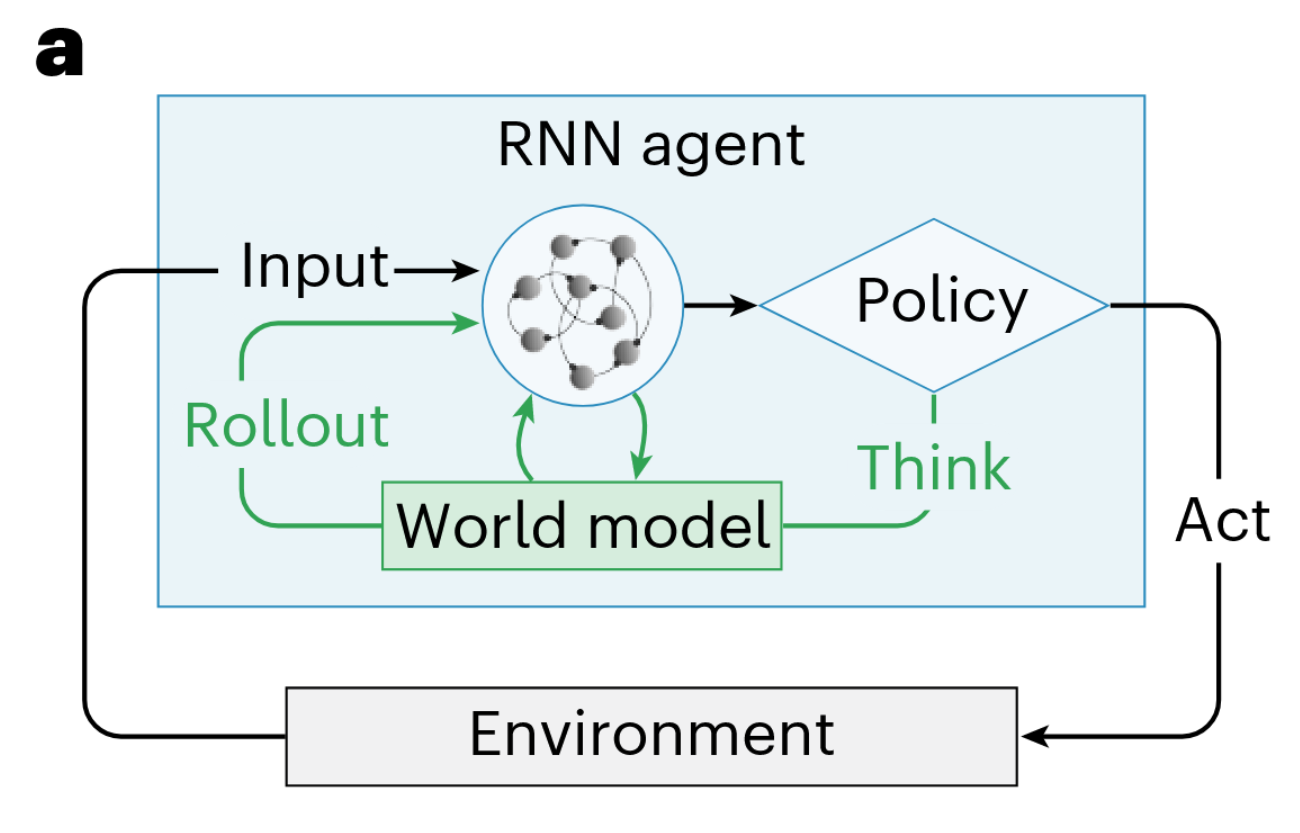
\includegraphics[scale=0.2]{figs/fig2.png}
	\centering
	\caption{模型工作流程示意图。}\label{fig:fig2}
\end{figure}

\subsection{本文实验范式概述(仅模型)}
\subsubsection{实验环境:} 
4×4的网格迷宫,具有周期性边界,存在不可穿越的墙壁和一个隐藏的奖励目标。

\subsubsection{实验流程:}
1. 每个实验周期(T = 20秒),模型进行移动消耗400ms,模型进行“思考”消耗120ms,包含多个试验。

2. 每个周期开始时,墙壁配置、奖励位置和初始位置随机抽取并固定,直到下一个周期。

3. 在每个周期的第一个试验中,agent通过在四个基本方向上离散移动来探索迷宫,直到找到隐藏的奖励。

4. 找到奖励后,agent立即被移动到一个新的随机位置,开始利用阶段,需要从随机起始位置反复返回到相同的目标位置。

\begin{figure}[H]
	\center
	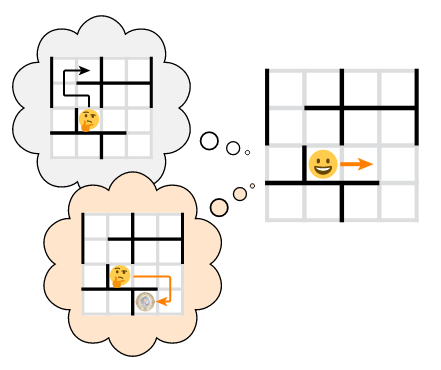
\includegraphics[scale=0.6]{figs/fanshi.png}
	\centering
	\caption{实验范式示意图。}\label{fig:fanshi}
\end{figure}

\subsection{Agent模块}
	这部分本人使用Pytorch对文章中的RNN agent进行复现。
	Agent模块是本文中元强化学习模型的核心部分,负责在环境中进行决策和规划。该模块基于循环神经网络(RNN)实现,能够通过采样自身的策略生成想象中的行动序列(称为“rollouts”)来进行规划。Agent模块的主要功能包括:

	1. 状态感知:接收环境的当前状态信息,包括位置、时间、墙的位置等。

	2. 动作生成:根据当前状态和内部策略生成动作。

	3. 内部规划:通过内部规划(rollouts)评估不同动作序列的潜在价值。

	4. 策略更新:根据环境反馈和内部规划结果更新策略。

\subsection{Env模块}
	这部分本人使用Gymnasium对文章中的Environment进行复现。
	Env模块是本文中环境的实现部分,负责模拟Agent所处的环境。该模块基于Gymnasium框架实现,能够生成环境的状态信息,并根据Agent的动作更新环境状态。Env模块的主要功能包括:
	
	1. 环境初始化:初始化环境的状态,包括位置、时间、墙的位置等。
	
	2. 状态生成:根据环境的当前状态生成新的状态信息。
	
	3. 动作处理:根据Agent的动作更新环境状态,并生成新的反馈信息。
	
	4. 环境反馈:生成环境的反馈信息,包括奖励、终止条件等。

\subsection{损失函数}


\begin{align*}
\mathcal{U} &= E_{E}[\rho(\theta)] \\
&= E_{E}[E_{x}(\sum_{k=1}^{K} r_{k})]
\end{align*}
在这里,$\mathcal{U}$ 是效用函数, $k$ 表示一个回合内的迭代次数, $r_{k}$ 表示每次迭代的即时奖励。我们还引入了以下辅助损失:
\begin{align*}
\mathcal{L}_V &= 0.5(V_k - R_k)^2 \quad \text{value function} \\
\mathcal{L}_H &= E_{n}[\log n] \quad \text{entropy regularization} \\
\mathcal{L}_P &= -\sum_{i} [s_{k+1}^{(i)} \log s_{k+1}^{(i)} + g^{(i)} \log g_{k}^{(i)}] \quad \text{internal world model}
\end{align*}
在这里,$\delta_{k} = -V_{k} + R_{k}$ 是“优势函数”, $\Delta\theta_{p} = \nabla_{\theta}\mathcal{L}_{p}$ 是预测损失$\mathcal{L}_{p}$的导数,用于训练“内部世界模型”。


最后我们得到了如下公式,更新模型参数:

\[
\Delta\theta \propto \sum_{a_k \sim \pi} \left[ \left( \underbrace{\nabla_{\theta} \log \pi_k(a_k)}_{\text{actor}} + \underbrace{\beta_{\nu} \nabla_{\theta} V_k}_{\text{critic}} \right) \delta_k - \beta_e \nabla_{\theta} \sum_a \underbrace{\pi_{k,a} \log \pi_{k,a}}_{\text{entropy}} + \underbrace{\beta_p \Delta \theta_p}_{\text{predictive}} \right]
\]


\section{复现细节}

\subsection{与已有开源代码对比}
	文章提供了Julia的源代码,本人使用Python进行复现。
	
	深度学习框架使用:Pytorch,强化学习框架使用:Gymnasium。

	由于文章工作量巨大,本人能力有限,仅复现了文章中心理学范式的场景和模型的训练,包括生成Agent和Environment,并对训练过程中Agent的部分行为结果进行了简单分析。

\subsection{创新点}
1. 在模型输入中,不仅考虑了传统的状态和动作信息,还引入了时间、墙的位置、计划缓存等多种模态的信息。这种多模态输入使得模型能够更全面地理解环境状态,从而做出更准确的决策。

2. 引入了动态规划模块(Planner),在每个时间步中,Agent不仅根据当前状态选择动作,还会进行一系列的内部规划(rollouts),以评估不同动作序列的潜在价值。这种内部规划机制使得Agent能够更有效地探索环境,提高决策的准确性。

\section{实验结果分析}
\subsection{参数}

1. R: 当前epoch中,模型获得的平均奖励的平均次数。

2. pred: 当前epoch中,模型对自身位置的预测的平均准确率。

3. plan: 当前epoch中,模型进行rollout,也就是“思考”的平均概率。

4. first: 当前epoch中,模型第一次到达目标位置时所花费的平均时间。

\subsection{分析}

1. 从图表和数据中可以看出,随着训练周期(epochs)的增加,奖励值整体呈现上升趋势。这表明代理在学习过程中逐渐优化其策略,能够获得更多的奖励。 

2. 预测值迅速上升并在短时间内达到稳定状态,这表明代理很快就能够准确地预测其行为的结果。预测能力的快速提升有助于代理在复杂环境中做出更合理的决策。

3. 模型的选择plan的概率稳步提升,说明模型策略的改变,即:随着训练的进行,模型有更高的概率通过内部世界的rollout操作,做出规划。

4. 第一次到达目标位置时所花费的平均时间,几乎没有任何变化,说明模型在探索阶段也和人类一般找到奖励的概率是随机的。


\begin{figure}[H]
	\center
	\includegraphics*[width=16cm]{figs/progress.png}
	\centering
	\caption{训练过程图}\label{fig:fig-progress}
\end{figure}

\begin{figure}[H]
	\center
	\includegraphics*[width=16cm]{figs/image-00.png}
	\centering
	\caption{训练数据-1}\label{fig:train-data-1}
\end{figure}

\begin{figure}[H]
	\center
	\includegraphics*[width=16cm]{figs/image-02.png}
	\centering
	\caption{训练数据-2}\label{fig:train-data-2}
\end{figure}

\begin{figure}[H]
	\center
	\includegraphics*[width=16cm]{figs/image-04.png}
	\centering
	\caption{训练数据-2}\label{fig:train-data-3}
\end{figure}


\section{总结与展望}
在模型实现方面,我们使用Pytorch复现了文章中的RNN agent,并使用Gymnasium复现了Environment。Agent模块负责状态感知、动作生成、内部规划和策略更新,而Env模块则负责环境初始化、状态生成、动作处理和环境反馈。我们还详细描述了损失函数的构成,包括效用函数、价值函数、熵正则化和内部世界模型的预测损失,这些损失函数共同指导模型参数的更新。

尽管本研究取得了一定的成果,但仍存在一些不足之处,未来的研究可以进一步探索以下几个方向:

1. 多模态信息的深度融合:虽然我们引入了多种模态的信息,但如何更有效地融合这些信息以进一步提高模型的决策能力仍是一个值得研究的问题。可以考虑使用更先进的多模态融合技术,如注意力机制或Transformer架构,来更好地处理和整合不同模态的信息。

2. 动态规划模块的优化:内部规划(rollouts)机制在提高决策准确性方面发挥了重要作用,但目前的实现可能还不够高效。未来可以探索更高效的规划算法,如蒙特卡洛树搜索(MCTS)或深度强化学习中的其他先进规划方法,以进一步提升模型的性能。

3. 模型的泛化能力:目前的模型在特定的实验环境中表现良好,但其泛化能力仍有待提高。可以考虑在更复杂的环境或不同的任务中测试模型的性能,以验证其在更广泛场景下的适用性。

4. 与人类行为的对比研究:虽然模型的某些行为与人类行为相似,但可以进一步深入研究模型与人类行为之间的具体差异和相似性。通过对比分析,可以更好地理解模型的机制,并为认知科学和神经科学提供更深入的见解。

5. 模型的可解释性:提高模型的可解释性是当前人工智能领域的一个重要研究方向。可以探索如何解释模型的内部规划过程和决策机制,使研究人员和实践者能够更好地理解模型的行为,从而提高模型的可信度和应用价值。

\bibliographystyle{plain}
\bibliography{refs.bib}

\end{document}